% master file siminos/froehlich/slice/intro.tex
% $Author$ $Date$

% \section{Introduction}
%    \label{sec:intro}

In spatially extended, turbulent flows one observes similar patterns at
different spatial positions and different times. How `similar?' If the
flow is equivariant under a group of continuous symmetries, one way of
answering this question is by measuring distances between different
states in the symmetry-reduced \statesp\ $\pS/\Group$, a space in which
each group orbit (class of physically equivalent states) is represented
by a single point. This `distance' depends on the choice of norm and on
the symmetry-reduction method. Our goal is to formulate a computationally
straightforward method of reducing continuous symmetries, applicable to
high-dimensional chaotic/turbulent flows, such as the translationally
equivariant fluid flows bounded by pipes or
planes\rf{GHCW07,GibsonMovies}. The literature (see
\refrefs{CBcontinuous,SiCvi10} for a review) offers two approaches (a)
invariant polynomial bases, and (b) methods which pick a representative
point by slicing group orbits, generalizing the way in which {\PoincSec}s
cut time-evolving trajectories. The \mslices\ studied in
\refrefs{SiCvi10,Wilczak09,CBcontinuous} offer a feasible approach,
implementable in practice. Here the method is rederived as a distance
minimization problem in the space of patterns.

We review basic facts
about symmetries of dynamical systems in \refsect{sec:SymmDyn}.
The new results reported in this paper are:
    (a) A generic linear slice cuts across group orbits of {\em all}
        states in the \statesp\ (\refsect{sec:frame}).
    (b) Every slice carries along with it a {\sset}. We show how to
        compute the jump of the \reducedsp\ trajectory
         (\refsect{sec:mslices}) whenever it crosses
        through such singularity  (\refsect{sec:singul}).
    (c) We propose to avoid these singularities (artifacts of the symmetry
        reduction by linear slices) by tiling the \statesp\ with an atlas
        constructed from a set of local slices  (\refsect{sec:chart}).
	(d) We show that if a continuous symmetry has a product structure
	   (such as $\SOn{2} \times \SOn{2}$ symmetries of pipe and plane
	   fluid flows), each symmetry induces its own {\sset} (\refsect{sec:??}).

\subsection{Symmetries of dynamics}
\label{sec:SymmDyn}

A flow $\dot{x}= \vel(x)$ is \emph{equivariant} under an coordinate
transformation $\LieEl$ if
\beq
\vel(x)=\LieEl^{-1}\vel(\LieEl \, x)
\,.
\ee{eq:FiniteRot}
The totality of group elements
$\LieEl$ forms \Group, the {\em symmetry group} of the flow. For
example, \KSe\rf{ku,siv,SCD07}, {\pCf}\rf{Visw07b,GHCW07,HGC08}, and
cylindrical pipe flow\rf{Wk04,Kerswell05} are equivariant under
combinations of translations and/or rotations. In numerical studies the
(non-compact) translation groups are rendered compact by the imposition of
periodic boundary conditions.

An element of a compact Lie group $\Group \subset \On{d}$ that is
continuously connected to the identity can be expressed as
\beq
\LieEl(\gSpace)=e^{{\gSpace} \cdot \Lg }
    \,,\qquad
\gSpace \cdot \Lg = \sum_{a=1}^N \gSpace_a \Lg_a
\,,
\ee{FiniteRot}
where $\gSpace \cdot \Lg $ is a \emph{Lie algebra} element, $\gSpace
= (\gSpace_1,\gSpace_2,\cdots\gSpace_N)$ are the parameters of the
transformation, and the $\Lg_a$ are a set of $N$ linearly independent
$[d\!\times\!d]$ antisymmetric matrices acting linearly on the {\statesp}
vectors. The group action parameters $\gSpace_a$ are often referred to as
`phases,' or `shifts.'
An infinitesimal group action is generated by
$
\LieEl(\delta \gSpace) \simeq 1 + \delta \gSpace \cdot \Lg
\,.
$ %\ee{eq:infinitesimal}
A corresponding spatial transformation induced by infinitesimal
variations of group `phases' $\delta \gSpace_a$ is
\beq
\delta {\ssp} = \delta \gSpace \cdot \groupTan(\ssp)
\,,
\ee{PC:groupTan0}
where the tangent vectors
\beq
 \groupTan_{a}(\ssp) = \Lg _{a} \ssp
    \,,\qquad
 a=1,2,\cdots,N,
\ee{PC:groupTan}
span the group tangent space at $\ssp$. We use $\groupTan_a(\ssp)$
notation (rather than $\Lg_{a}\ssp$) to emphasize that the group action
induces a \emph{tangent field} at $\ssp$.

Any representation of a compact group $\Group$ is fully
reducible. The invariant tensors constructed by contractions
of $\Lg_a$ are useful in identifying irreducible
representations. The simplest such invariant is
\beq
{\Lg} \cdot \Lg = - \sum_m C_2^{(m)} \, \id^{(m)}
\,,
\ee{QuadCasimir}
where $C_2^{(m)}$ is the quadratic Casimir for irreducible representation
labeled $m$, and $\id^{(m)}$ is the identity on the $m$-irreducible
subspace, 0 elsewhere. For compact groups $C_2^{(m)}$ are strictly
nonnegative. $C_2^{(m)} =0$ if $m$ is an invariant subspace.

    %
% \subsection{\SOn{2} irreducible representations.}
%   \label{exam:SO2irrepst}
    %
The simplest example of a Lie group is given by the action of \SOn{2} on
a smooth function $u(\gSpace + 2\pi) = u(\gSpace)$ periodic on interval
$[-\pi,\pi]$. Expand $u$ as a Fourier series
\beq
u(\gSpace) = \frac{a_0}{2} + \sum_{m=1}^\infty \left(
a_m \cos m \gSpace + b_m \sin m \gSpace
                               \right)
\,.
\ee{FourierExp}
The matrix representation of the \SOn{2}\ action
$\LieEl(\gSpace') u(\gSpace) = u(\gSpace+\gSpace')$
on the Fourier coefficient pair
$(a_m,b_m)$ is
\bea
\LieEl^{(m)}(\gSpace')
    &=& \exp{\left({\gSpace} \cdot \Lg^{(m)}\right)}
	\,=\,
   \left(\barr{cc}
 ~\cos m \gSpace'  & \sin m \gSpace' \\
 -\sin m \gSpace'  & \cos m \gSpace'
    \earr\right)
\continue
&=& \cos m \gSpace' \id^{(m)}
  + \sin m \gSpace'\, \frac{1}{m} \Lg^{(m)}
\,,
\label{SO2irrepAlg-m}\\
 \Lg^{(m)} &=&   \left(\barr{cc}
    0  &  m  \\
   -m  &  0
    \earr\right)
\,.
\label{SO2irrepAlg-Lg}
\eea
$\Lg^{(m)}$ is the Lie algebra generator and $\id^{(m)}$ is the identity
on the irreducible subspace labeled $m$, 0 elsewhere. The \SOn{2}\ group
tangent $\groupTan(u)$ to \statesp\ point $u$ is
\beq
 \groupTan(u) = \sum_{m=1}^\infty \groupTan^{(m)}(u)
    \,,\qquad
 \groupTan^{(m)}(u)
\,=\, m \,\left(\barr{c}
   ~b_m  \\
   -a_m
    \earr\right)
\,.
\ee{u:x:tang}
	
We shall illustrate symmetry reduction by applying it to the \cLe\
\bea
	\dot{x}_1 &=& -\sigma x_1 + \sigma y_1
\continue
	\dot{x}_2 &=& -\sigma x_2 + \sigma y_2
\continue
	\dot{y}_1 &=& (r_1-z)\, x_1  - ~y_1 - e y_2
\continue
	\dot{y}_2 &=& (r_1-z)\, x_2 + e y_1 - ~y_2
\continue
	\dot{z}~ &=& -b z + x_1 y_1 + x_2 y_2
\,.
\label{eq:CLeR}
\eea
They were introduced by Gibbon and McGuinness\rf{GibMcCLE82}
as a 5-dimensional model of baroclinic instability in the
atmosphere.
In all numerical calculations that follow we shall set the
parameters to \refref{SiCvi10} values,
\beq
r_1=28,\; b={8}/{3},\;
\sigma=10,\quad \mbox{and}  \quad e={1}/{10}
\,,
\ee{SiminosPrmts}
for which \cLe\ exhibits a strange attractor,
\reffig{fig:Fullspace}.

 \begin{figure}
 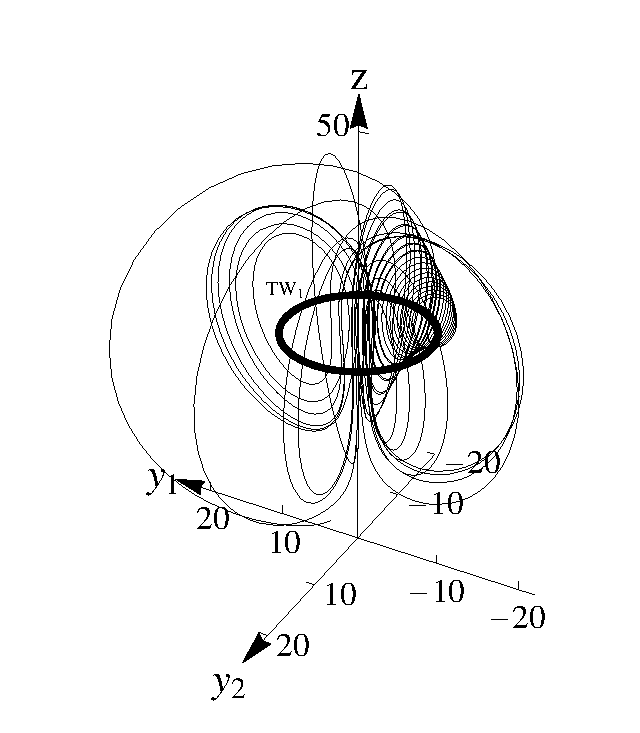
\includegraphics[width=0.35\textwidth]{Fullspace}%
 \caption{\label{fig:Fullspace}
\CLe\ \refeq{eq:CLeR} exhibit a strange attractor for
parameter values \refeq{SiminosPrmts}. (thin line)
A segment of generic finite time trajectory. (thick line)
$\REQV{}{1}$, the only \reqv.
 }%
 \end{figure}

\CLe\ are a simple example of a dynamical system
with a continuous (but no discrete) symmetry.
They are equivariant under
finite angle \SOn{2} rotations given by
\beq
\LieEl(\gSpace) \,=\,  \left(\barr{ccccc}
  \cos \gSpace  & \sin \gSpace  & 0 & 0 & 0 \\
 -\sin \gSpace  & \cos \gSpace  & 0 & 0 & 0 \\
 0 & 0 &  \cos \gSpace & \sin \gSpace   & 0 \\
 0 & 0 & -\sin \gSpace & \cos \gSpace   & 0 \\
 0 & 0 & 0             & 0              & 1
    \earr\right)
\,.
\ee{CLfRots}
The corresponding Lie algebra generator is
\beq
 \Lg \,=\,   \left(\barr{ccccc}
    0  &  1 & 0  &  0 & 0  \\
   -1  &  0 & 0  &  0 & 0 \\
    0  &  0 & 0  &  1 & 0  \\
    0  &  0 &-1  &  0 & 0 \\
    0  &  0 & 0  &  0 & 0
    \earr\right)
\,.
\ee{CLfLieGen}
The group is 1\dmn\ and compact, its
elements parameterized by $\gSpace \mbox{ mod } 2\pi$.
The action of \SOn{2}\ thus decomposes the  \statesp\ into $m=0$
\SOn{2}-invariant subspace ($z$-axis) and  $m=1$ subspace of
multiplicity 2. Locally, at
\statesp\ point $\ssp$, the infinitesimal action of the group is
given by the group tangent field $\groupTan(\ssp) = \Lg \ssp
= (x_2,-x_1,y_2,-y_1,0)$, with the flow induced by
the group action normal to the radial direction in the
$(x_1,x_2)$ and $(y_1,y_2)$ planes, while the $z$-axis is left
invariant.

%
% ****** End of file intro.tex ******
